\documentclass[german, master, utf8, pdftex, dvipsnames]{base/thesis_KBS}

\usepackage{units}    % \unit[23]{m}
\usepackage{nicefrac} % \nicefrac{km}{h}
\usepackage{environ}
\usepackage[justification=centering]{subcaption} % mehrere Bilder in einer figure
\usepackage{pgfplots} % Plots für Benchmarks
\usepackage{csquotes} % Anführungszeichen
\usepackage{float} % figure platzieren
\usepackage{listings} % Code einfügen
\usepackage{tabto} % Einrückung zu einer festen Position
\usepackage{pdfpages} % Einfügen der Erklärung am Ende
\usepackage[shortlabels]{enumitem} % Mehr Optionen für enumerate
\usepackage{xfrac} % Bessere Brüche
\usepackage{booktabs} % Bessere Tabellen
\usepackage[protrusion=false,spacing=true]{microtype} % Bessere Text Skalierung
\usepackage{subfiles} % include
\usepackage{silence} % Unterdrückung von Warnungen
\usepackage[figuresright]{rotating} % Bilder rotieren
\usepackage{amsmath}
\usepackage{makecell}
\newcommand*\colvec[1]{\begin{pmatrix}#1\end{pmatrix}}

\usepackage{xargs}                      % Use more than one optional parameter in a new commands
%\usepackage[pdftex, dvipsnames]{xcolor}  % Coloured text etc.
\usepackage{xcolor}
% 
\usepackage[colorinlistoftodos,prependcaption,textsize=tiny]{todonotes}
\newcommandx{\unsure}[2][1=]{\todo[linecolor=orange,backgroundcolor=orange!25,bordercolor=orange,#1]{#2}}
\newcommandx{\change}[2][1=]{\todo[linecolor=blue,backgroundcolor=blue!25,bordercolor=blue,#1]{#2}}
\newcommandx{\info}[2][1=]{\todo[linecolor=green,backgroundcolor=green!25,bordercolor=green,#1]{#2}}
\newcommandx{\improvement}[2][1=]{\todo[linecolor=red,backgroundcolor=red!25,bordercolor=red,#1]{#2}}
\newcommandx{\thiswillnotshow}[2][1=]{\todo[disable,#1]{#2}}

\usepackage{algorithm, algorithmic}  % for pseudo code (cf. documentation)
\renewcommand{\algorithmiccomment}[1]{\qquad{\small // \textit{#1}}}

\pgfplotsset{compat=1.16} % pgfplots config
\setquotestyle{american} % csquotes config
\raggedbottom % verhindert Lücken zwischen Überschriften und Text
\hyphenpenalty=750 % macht Worttrennung seltener

\NewEnviron{myequation}{	
	\begin{equation}
		\scalebox{1.2}{$\BODY$}
	\end{equation}
}

\newcommand{\norm}[1]{\left\lVert#1\right\rVert}
	

\WarningFilter*{microtype}{I cannot find}

% verhindert (meistens) Zeilenumbrüche vor Verweisen
%\NewCommandCopy{\oldref}{\ref}
%\renewcommand{\ref}[1]{\nolinebreak \oldref{#1}}
%\NewCommandCopy{\oldcite}{\cite}
%\renewcommand{\cite}[1]{\nolinebreak \oldcite{#1}}

\newcommand{\pleasedontaddwhorechildren}{\newpage}

\lstset{
    basicstyle=\ttfamily\small,
    numberstyle=\footnotesize,
    numbers=left,
    backgroundcolor=\color{gray!10},
    frame=single,
    tabsize=2,
    rulecolor=\color{black!30},
    title=\lstname,
    escapeinside={\%*}{*)},
    breaklines=true,
    breakatwhitespace=true,
    framextopmargin=2pt,
    framexbottommargin=2pt,
    showstringspaces=false
    inputencoding=utf8,
    extendedchars=true,
    literate={ä}{{\"a}}1 {ö}{{\"o}}1 {ü}{{\"u}}1 {ß}{{\ss}}1 {∆}{{$\Delta$}}1,
}

%%%%%%%%%%%%%%%%%%%%%%%%%%%%%%%%%%%%%%%%%%%%%%%%%%%%%%%%%%%%%%%%%%%%%%%%%%%%%%%

\begin{document}

\title{Loop Closure in TSDF basiertem SLAM} % Deckblatt
\shorttitle{Loop Closure in TSDF basiertem SLAM} % Für Titel am unteren Rand der Seiten

\author{Patrick Hoffmann}
\email{pahoffmann@uni-osnabrueck.de}
\firstSupervisor{Prof. Dr. Mario Porrmann}
\secondSupervisor{Alexander Mock}
% \submitdate{August 2022}             % by default current month & year
%signline{Osnabrück, 11. Dezember 2004} % by default "signcity, submitdate"

\generatetitle

\cleardoublepage

\begin{prefacesection}{Zusammenfassung}

Die vorliegende Arbeit beschäftigt sich mit der Implementierung und Konzeption einer Lösung zur Detektion von \textbf{Schleifenschlüssen} in einem auf \textbf{Truncated Signed Distance Funtion (TSDF)} basierenden \textbf{Simultaneaous Localization and Mapping (SLAM)} Ansatz und der nachfolgenden Optimierung der Robotertrajektorie und TSDF-Karte.
Zur Optimierung der Trajektorie des Robters nach der Identifikation eines Schleifenschlusses kommt die Bibliothek \textbf{GTSAM} zum Einsatz.
Es wird evaluiert ob und unter welchen Voraussetzungen eine Nachbearbeitung auf Basis einer fertigen TSDF Karte mit zugehöriger initialer Trajektorie möglich ist und zusätzlich der Einsatz in einem inkrementellen SLAM Ansatz geprüft.
Darüber wird untersucht, inwiefern ein Teilupdate der TSDF basierten Karte möglich ist.

\end{prefacesection}

\vspace{5cm}

\begin{prefacesection}{Abstract}

This paper deals with the implementation and design of a solution for the detection of \textbf{loop closures} in a \textbf{Truncated Signed Distance Function (TSDF)} based \textbf{Simultaneaous Localization and Mapping (SLAM)} approach and the subsequent optimization of the robot trajectory and TSDF map.
The \textbf{GTSAM} library is used to optimize the robot's trajectory after identifying a loop closure.
It is evaluated whether and under which conditions a postprocessing based on a finished TSDF map with associated initial trajectory is possible and additionally the use in an incremental SLAM approach is examined.
Furthermore, it will be investigated to what extent a partial update of the TSDF based map is possible.

\end{prefacesection}


\cleardoublepage
\tableofcontents


\startTextChapters %%%%%%%%%%%%%%%%%%%%%%%%%%%%%%

% Einleitung + Motivation
\subfile{chapters/einleitung}

% Stand der Technik
\subfile{chapters/standdertechnik}

% verwendete libraries
%\subfile{chapters/libraries}

% tsdf, slam, loop closure
\subfile{chapters/grundlagen}

\subfile{chapters/daten_assoziationen}

\subfile{chapters/loopclosure}

\subfile{chapters/map_update}

\subfile{chapters/ausblick}


\bibliography{papers.bib}                                                                                                                           

\cleardoublepage

\improvement{Endpage für Unterschrift einbauen}
%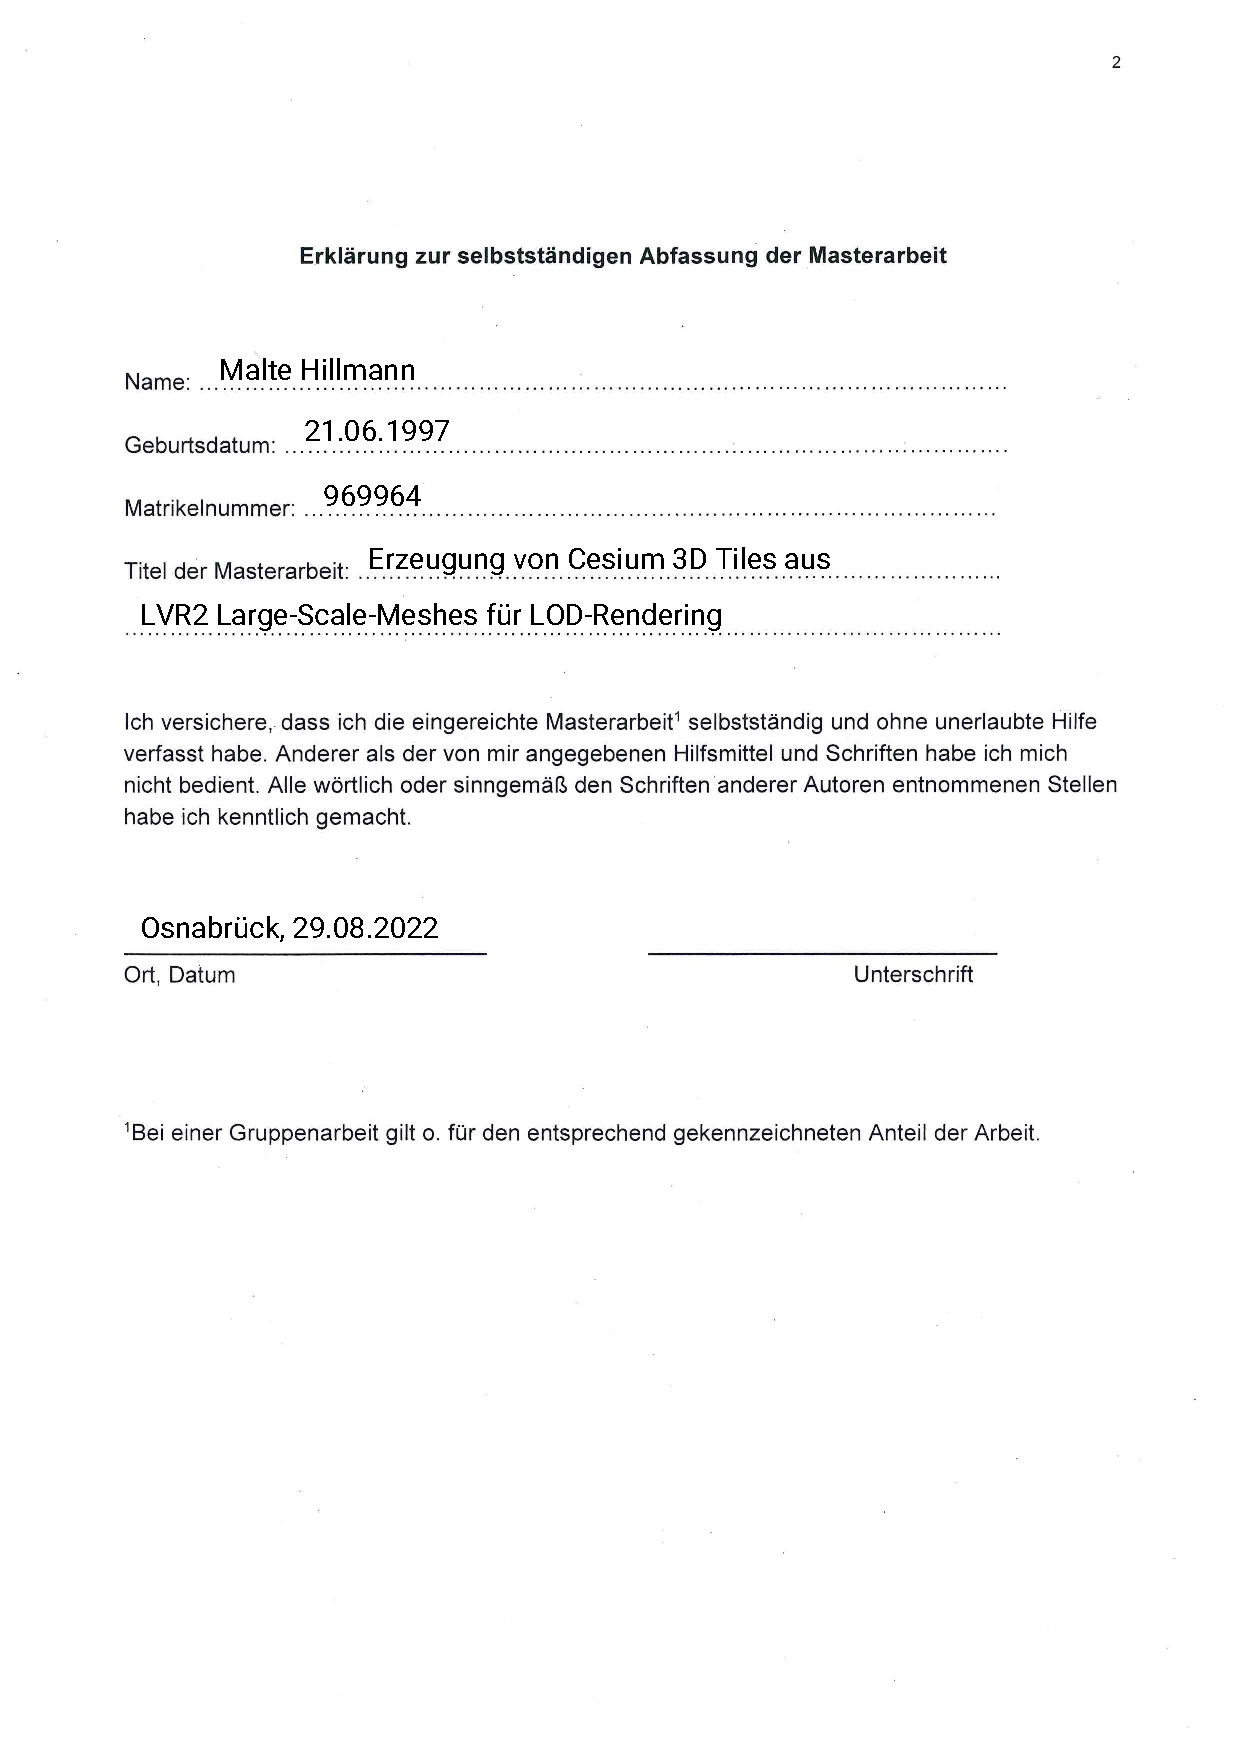
\includepdf[pages=-]{pics/endpage.pdf} %%%%%%%%%%%%%%%%%%%%%%%%%%%%%%

\end{document}
